\chapter{Introduction}

Deefake is the buzzword that has no agreed-upon technical definition. It consists of two words, deep and fake. Deep is referring to deep learning machine learning, which is used for creating fake voices, images, or even videos. It is a fast growing technical field of study and could be a major threat to society. We live in information era and creation of unrecognizable fake media affects us all. Deepfakes could be found on social media, news portals, etc.

This paper shows some security risks and impacts on many different fields of human life. There are already several successful attacks on biometrics systems, and many popular videos containing deepfakes on social networks with millions of views. People are not able to consistently recognize deepfakes. That is why we need to create detection tools to help anyone with problem that is already there.

There are many different deepfake categories from face swap to face morphing and more. Most of the detection methods focus on a single domain, which means that they are capable of detecting only one deepfake category. There are few tools in the market targeting undemanding/inexperienced users, and some of them are not free to use.

The first two chapters cover general knowledge about deepfakes such as potential risks and security impacts with mention of successful attacks, different types of voice, image, and video deepfakes. You can read about experimental detection methods and available tools in the market.

Second and more important part describes process of development deepfake detection framework and client application, which is the goal of this work. It starts by specifying requirements followed by detailed architecture. Architecture was designed with focus to easily integrates new detection methods into framework.

Last but not least, the implemented framework containing several open source detection methods was deployed into Azure AKS cluster and properly tested. The tests were mostly focused on the testing framework itself, mostly measuring used resources. Integrated detection methods were also tested, and all the results could be found at the end of this paper.

\chapter{Security impacts of deepfakes}

The creation of fake media and their detection have been a problem since photography was invented. Digital photography or video with tools such as GIMP, Adobe Photoshop or Adobe After Effects allows more people to create fakes than before, still some experience in this area is needed. Media that have been modified or otherwise manipulated are called synthetic media, and they do not depend on whether it is an analogue or digital medium. Deepfakes also fall under this category~\cite{IncreasingThreatofDeepfakeIdentites}. Deep learning-powered tools allow unexperienced users to easily create trusted fakes. 

The quality of deepfakes reached a level when a trained person or even an experienced researcher in this field has a problem of spotting them. This fast development allows creating realistically looking assets to art photography or movie production; unfortunately, it can be used for malicious purposes like creating fake porn videos to blackmail people or manipulate public via fake news. There are many use cases where deepfakes can be applied.

This is not a discussion about potential technology; deepfakes are already there and their usage will probably have an increasing trend. Over the last couple months, we could see huge development and popularity explosion around large language models such as ChatGPT~\cite{ ChatGPTPopularity}. Deepfakes do not have such publicity, but they have the same potential to change whole human society as previously mentioned language models. We are not far from using a pre-trained voice deepfake model powered by some large language model to automatically perform attack itself.

It is putting huge pressure on researchers to develop new forensics tools or any technology which will prevent malicious usage of deepfakes. As mentioned before, creating fakes is not new, and a whole field of study engaged in spotting fakes and developing techniques over 15 years. Despite continuous research efforts in the past, the advent of deep learning changed the rules of the game.~\cite{MediaForensicsandDeepFakes}

\section{Human capabilities of deepfake detection}

The human ability to recognize fake materials from the originals is in contradiction to their quality. Korshunov and Marcel \cite{TheThreatOfDeepfakes} confirmed this in their research. They created a questionnaire containing several videos, and the subject (interviewee) had to answer after watching the video whether the person in the video was genuine, fake, or uncertain. The videos were manually divided into five categories (very easy, easy, moderate, difficult, and very difficult, original). 

The videos were split into several categories manually by the researchers, probably without using any metrics but based on their experience and feelings. Afterwards, ANOVA test shows there is an overlap in several categories, so several videos could be moved to a different category. However, the categories are still significantly different.

The results of test in Fig. \ref{fig:subjective_answers} certainly demonstrate that people's recognition ability decreases significantly as the quality of deepfakes increases. Also, the audience of this test knows they are looking for fakes, otherwise we can expect worse results if there will be unsuspected audience (e.g., deepfakes on social media). It is quite alarming that the correct answers in the category of “very easy” reach only 71,1 \%. The quality of deepfake increases over time, thus it can be expected that human recognition ability will continue to decrease. \cite{TheThreatOfDeepfakes}

\begin{figure}[H]
    \begin{subfigure}[h]{0.4985\linewidth}
        \centering
        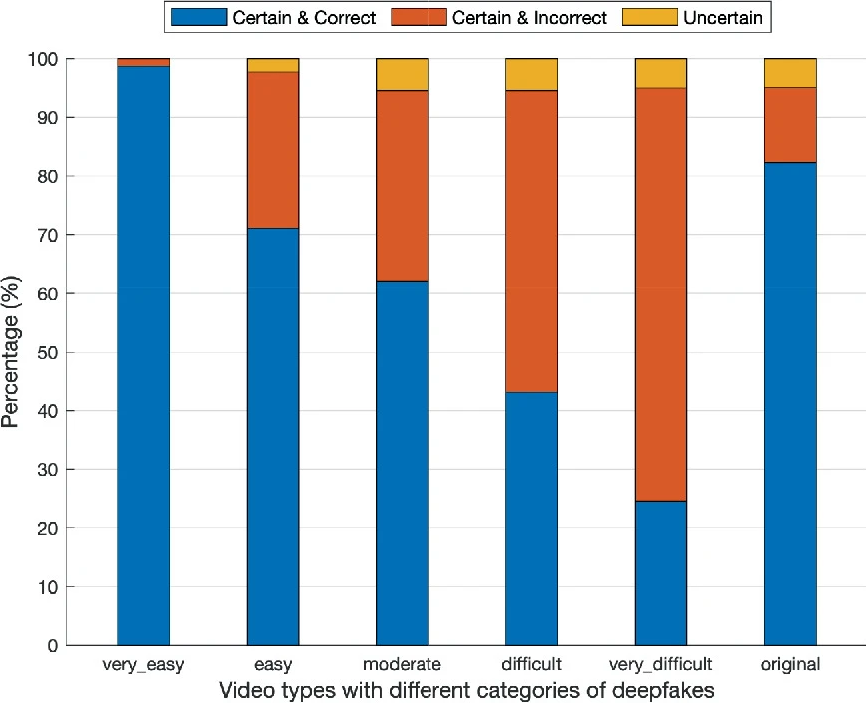
\includegraphics[width=1\linewidth]{other-fig/subjective_answers_a.png}
        \caption{Subjective answers}
    \end{subfigure}
    \hfill
    \begin{subfigure}[h]{0.4985\linewidth}
        \centering
        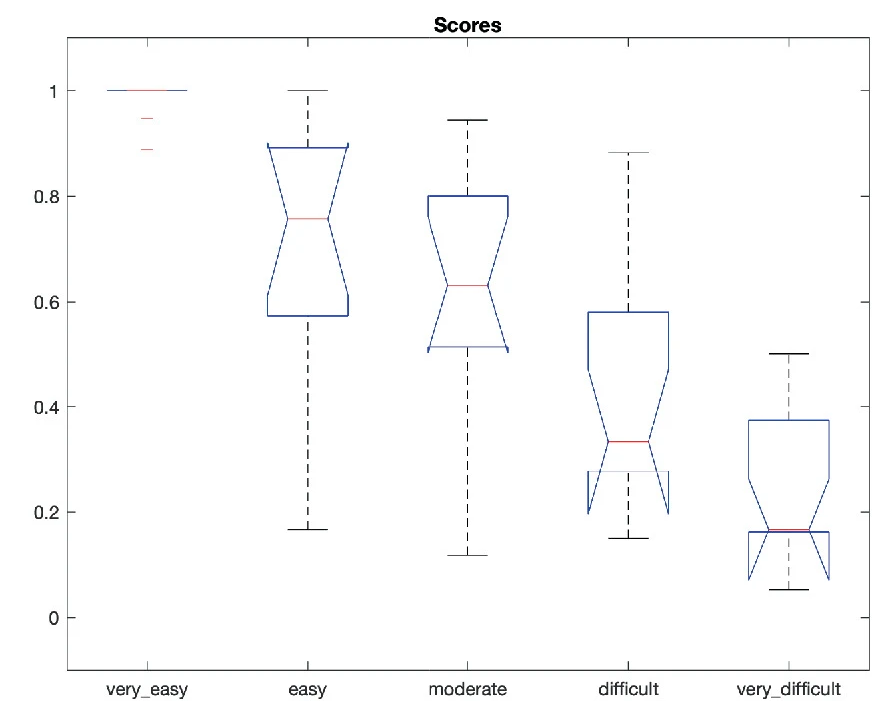
\includegraphics[width=1\linewidth]{other-fig/subjective_answers_b.png}
        \caption{ANOVA test}
    \end{subfigure}
    \caption{Subjective answers and median values with error bars from ANOVA test for different deepfake categories. Retrieved from~\cite{TheThreatOfDeepfakes}.}
    \label{fig:subjective_answers}
\end{figure}

Another research tested only recognition of audio tracks and they were comparing humans versus computer programs. Attendees had a correct classification between fakes and origins 67 \% after the first several rounds. Their accuracy increased while listening and answering to more tracks, but the value stabilizes at 80 \%. On average, trained AI performs about 10 \% better than human, but this result highly depends on the difference in learning and test dataset. Still, it shows that the computer can outperform humans in spotting deepfakes. \cite{HumanPerceptionAudio}

\section{Potentional risks and impacts}

Humans are not good at recognizing deepfakes, but “why should we be worried?”. Almost every technology humankind created could be used for good or bad – deepfake is no exception. There are plenty different deepfake categories, and each has its own attack vector or use case. This section is covering potential risks of those categories and their closer description will be covered in Chapter~\ref{chapter:deepfakes_creation}.

Deepfakes are about gaining someone’s trust or influencing him. For the last couple of years, there has been an increasing trend of scamming people, mostly via phone or computer~\cite{HybridVishingAttacksSkyrocketing}. Targeting only one person/victim, for example, to gain their money or information. Those attacks are getting better and more credible and using deepfake to impersonate close friend of victim could be next step how to improve it, if it is not already happening.

Creating “fake news” to influence a large audience is the most common use case of deepfakes because we live in an information era. There are many targets of “fake news” such as rigging elections, demoralizing military units, or manipulating the stock market. In this case, politicians, celebrities, and significant personalities will be used in deepfakes to influence the audience. We can only imagine what one person or a high quality deepfake can change with enough media reach. For example, after one tweet from Elon Musk about Tesla’s stock, sends shares down more than 10 \% almost immediately~\cite{ElonMusksTweets}.~\cite{IncreasingThreatofDeepfakeIdentites}

A real example of deepfake is the famous video with Barak Obama insulting Donald Trump, which should spread awareness regarding the fast developing category of new thread \footnote{\url{https://www.buzzfeed.com/craigsilverman/obama-jordan-peele-deepfake-video-debunk-buzzfeed}}. Several years later another video stating Volodimir Zelenskyj talking about surrendering, it was proved that it is a manipulated video, and its purpose was to demoralize Ukraine army and make them capitulate \footnote{\url{https://www.youtube.com/watch?v=X17yrEV5sl4}}.

There are other videos similar to the video of Barac Obama with the same purpose, spreading awareness about deepfake. For example speech of Czech Republic president Miloš Zeman created by HBO for also propagating their new series \footnote{ https://www.youtube.com/watch?v=FzMnDwpKJrI }. We can consider those videos and their goal to be mostly success. Most people have heard about deepfakes and they are connecting them with those types of videos. Most people heard about deepfakes and they are connecting them with those types of videos. However, many people share deepfakes inadvertently on their social media~\cite{DeepfakeSharing}.

Not everyone considered them as a big thread. This is probably because there is no proof that there was a successful deepfake attack or fake news that influence them directly. This is the reason why deepfake could be so dangerous. The video of Volodimir Zelenskyj might have had a good chance to be successful, but it was quite fast debunked because of its terrible deepfake quality. People still should inform about capabilities of deepfakes, and the target of the message should be different. Not saying only be careful we can make politicians say what we want but show and provide some tools on how to spot the deepfakes.

Another field where deepfakes could be used is to tricky biometrics systems in which the attacker is a different person to gain access (banking, building, etc.) to secured equipment, etc. Biometrics systems have been proven not ready to deal with deepfakes~\cite{DawnOfTextDependentSociety}~\cite{TheMagicPassport}. The work describing one of attacks is called magic passport and demonstrates how biometric systems could be vulnerable. Most systems will require some changes such as adding a new module to the authentication pipeline, which will be detecting deepfakes~\cite{DigitalFaceManipulation}. Face or voice biometrics recognition systems are in greatest danger. Falsification of documents is related to this topic and there was a case of smuggling people across borders with an official passport containing morphed photos of two individuals~\cite{FaceMorphingAttackDetectionMethods}.

These cases are only the tip of the iceberg, and in the future, everyone should ask if video on social media with film celebrities is real or even worse, if the evidence in courts is trustworthy or not. The solution to this is to use tools capable of detecting deepfakes. Those tools must be created with caution for unskilled users.

\section{Detection tools requirements}

Now we know that deepfakes could be security threats and there is a need for reliable detection tools. There is not many detection tool available for users. Most of them are basically command line scripts which are not for general purpose. More about individual methods could be fined in Chapter~\ref{chapter:deepfake_detectoin}.

The user interface should be simple, yet provide all relevant information. Generalizing anything to one number will be great, but not every time it is possible. Speaking of detection methods it should be able to deliver only one number. On the other hand, it will be nice to show the user where on the image is the manipulated area. 

Nowadays people work with many different types of files. Only for audio we can have WAV, OGG, MP3 and many more. This means that the detection method supporting only one file type will not have huge success. There are two types of solution to this problem; first is to support as many file types as possible natively. The second approach will be to utilize existing tools to convert input files to one specific format.

In the end how do we compere different detection methods or even the same methods trained on different datasets. We would have to test each method individually and compare the results manually. There are some problems that need to be sorted out before we will have a reliable detection tool in the market. 

\chapter{Types of deepfakes}
\label{chapter:deepfakes_creation}

There are plenty of methods on how to create deepfakes, and as its name suggests some of them are based on deep neural networks, but not exclusively. This section describes most common types of learning networks used for creating image/video or voice deepfakes. One of the most popular types for face deepfakes is Generative adversarial network (GAN), and it is used to create completely new faces or face manipulations.

Each method leaves traces in the medium that can then be detected. This is one way to recognize deepfakes so understanding process of creation is an advantage. Detecting will be described in more detail in Chapter~\ref{chapter:deepfake_detectoin}.

\subsection{Neural networks}

Neural networks are composited from neurons arranged in layers, and each layer is connected sequentially via synapses. Synapses are weighed, and the process of finding the proper value of all weights is called a learning neural network. To obtain results from the input of \(n\)-dimensional \(x\) process \texttt{forward-propagation} is used to propagate \(x\) through each layer.

Input to layer is vector \(a\) of values calculated by previous layer or in case of first layer \(x\) itself. That means result of each layer is also vector calculated by activation function \(f(a*W+b)\), where \(f\) is activation function (Sigmod, ReLU, etc.), \(a\) is input vector, \(W\) is matrix of weights between layers \(i\) and \(i+1\) and b is dimensional bias. Dimensional bias is a constant offset that helps the network shift the activation function toward the positive or negative side~\cite{NeuralNetworkBias}.

Now let’s consider the neural network \(M\) as a black box and denote its execution as \(M(x) = y\). Supervise learning to train \(M\) is using paired samples with from \((x_i, y_i)\) and loss function \(L\) is defined. Loss function is to generate a signal at the output of \(M\) and propagate him back to find error of each weight in synapses.

Optimalization algorithms such as gradient descent are then used to calculate new weights of \(M\) for the number of epochs. As a result of this process, the network learns the function \(M(x_i) \approx y_i\) and is capable of making prediction on unseen data. More detailed descriptions of this could be found in the work of Y. Mirsky and W. Lee~\cite{CreationandDetectionofDeepfakes}. ~\cite{CreationandDetectionofDeepfakes}
\\\\
Next list shows types of neural networks used for generating deepfakes~\cite{CreationandDetectionofDeepfakes}:

\begin{itemize}
\item Generative Adversarial Networks (GAN) – Consist of two neural networks working against each other. One layer is generator and second is discriminator. Generator producing fake features trying to fool discriminator, on the other hand, discriminator is learning to distinguish between real sample and fake one.
\item Encoder-Decoder networks (ED) – Contains at least two networks, encoder and decoder. It has narrowed layers towards its center. If encoder \(En\) and decoder \(De\) are symmetric and they are trained as \(De(En(x)) = x\), then the network is called autoencoder. Generating deepfakes using ED trained with function \(De(En(x)) = x_g\), where \(x_g\) is fake generated features. There is possibility to use multiple different ED chained after each other or using specific variant of ED called variational autoencoder.
\item Convolutional Neural Network (CNN) – CNN is learning pattern hierarchies in the data. For deepfakes purposes, it learns filters applied over the input and forming an abstract feature map as the output.
\item Recurrent Neural Networks (RNN) – RNN can handle variable length data and it is remembering stat after processing which can be used in next iteration. RNN are mostly used in audio.
\end{itemize}

Each architecture has its own subcategories that have small modifications or using some techniques from different architecture. All above mentioned neural networks types are shown in~\ref{fig:nns_architecture} and~\ref{fig:cnn_architecture} 

\begin{figure}[H]
    \centering
    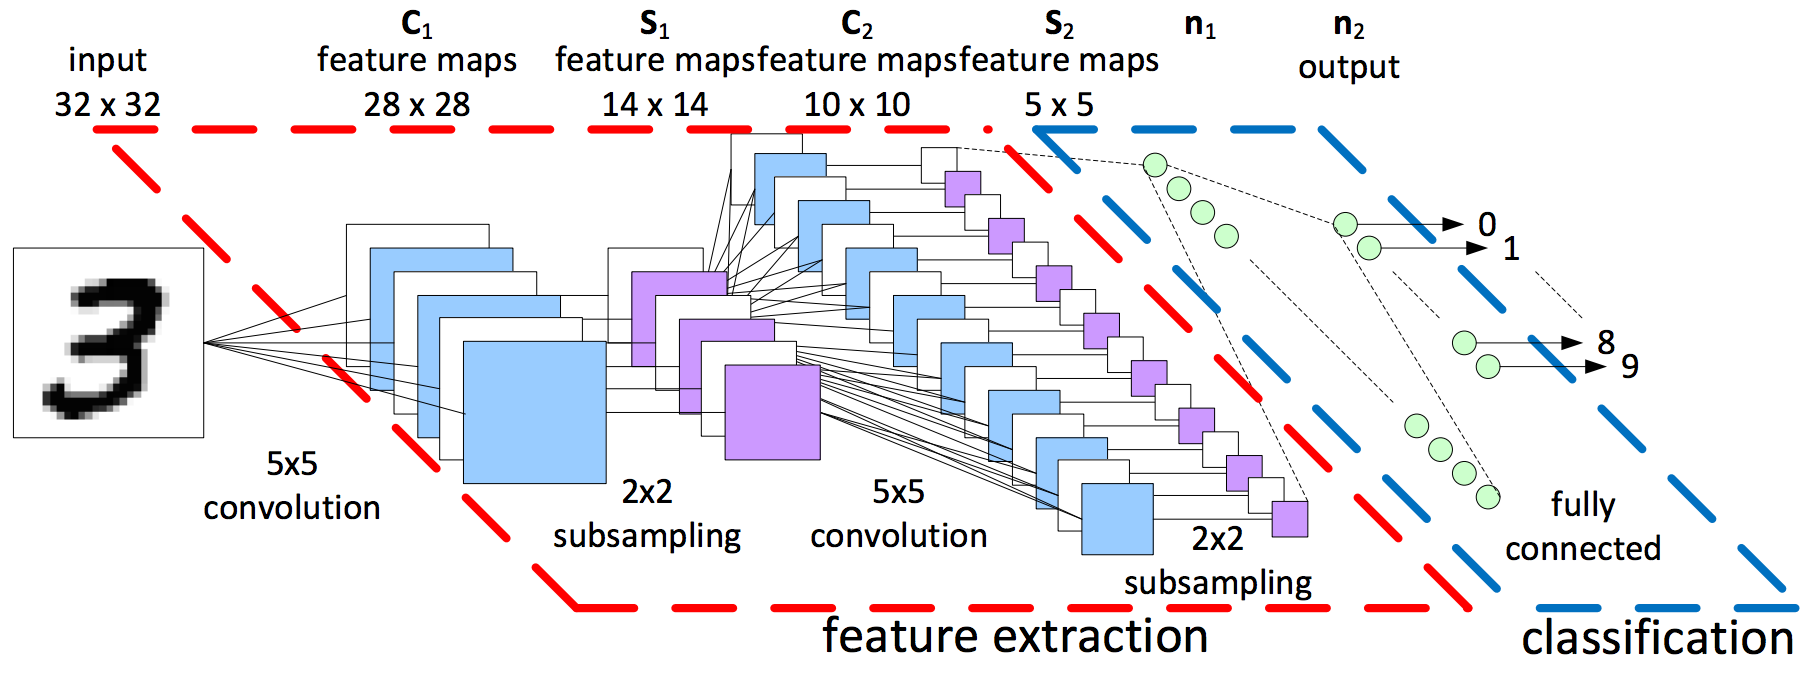
\includegraphics[width=.7\linewidth]{other-fig/cnn.png}
    \caption{Architecture of convolutional neural network. Retrieved from~\cite{CNNArchitecture}.}
    \label{fig:nns_architecture}
\end{figure}

\begin{figure}[H]
    \centering
    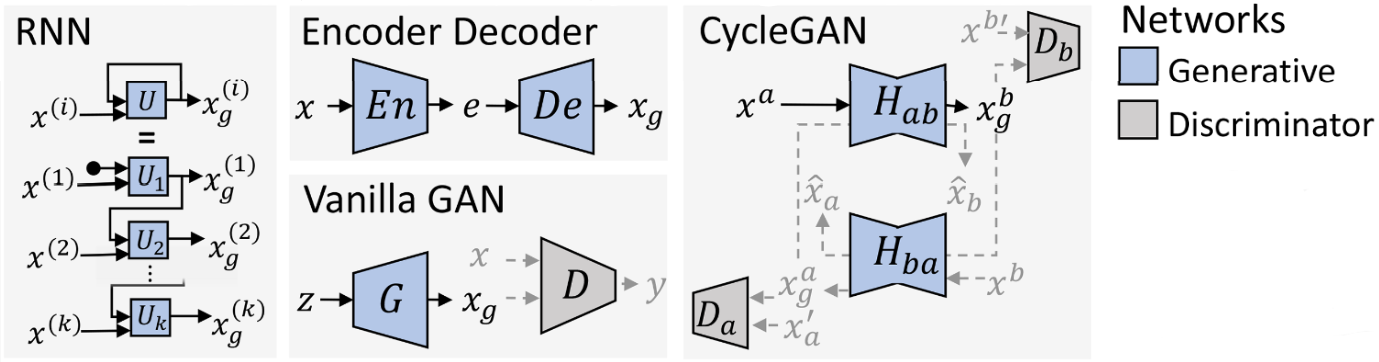
\includegraphics[width=.65\linewidth]{other-fig/nns.png}
    \caption{Basic neural network architectures (RNN, ED, GAN). Retrieved from~\cite{CreationandDetectionofDeepfakes}.}
\label{fig:cnn_architecture}
\end{figure}

\subsection{Voice deepfakes}

There are three different modalities for speech synthesis: text-to-speech (TTS), voice cloning (VC), and replay attack (RA).~\cite{Deepsonar} The last fine is based on the capture victim voice and the replay of it. It is quite easy and cheap to perform because it only requires capture and replay device (today we can use for example smartphone) and current methods for voice recognition still have accuracy issues.~\cite{ReplayAttackDetection} First two are using AI-synthesis with content regeneration which makes them more indistinguishable for naked ears.~\cite{Deepsonar}

Text to speech (TTS) converts written text to artificial speech, on the other hand voice cloning consumes source voice. Both methods produce synthesis voice saying desired phrases specified by the input, high-level diagram how those methods works could be seen on Fig.~\ref{fig:tts_vs}. Voice deepfakes are used independently or with deepfake video (e.g. full puppet). Creating synthesis voice is computationally challenging and one of the goals is making real-time voice cloning. There are several projects that are trying to accomplish this 3 4.

\begin{figure}[H]
    \centering
    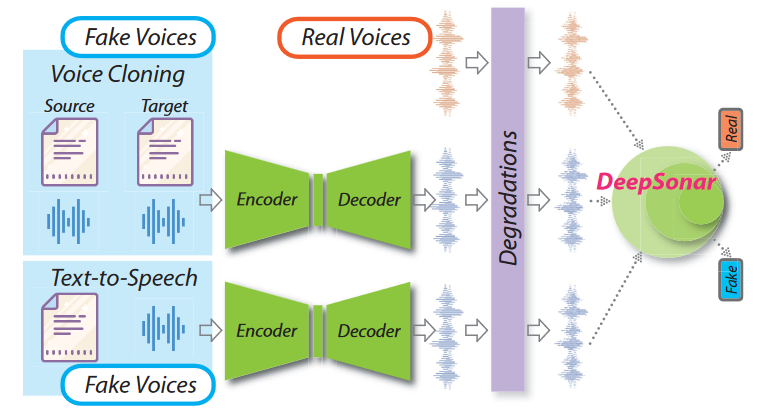
\includegraphics[width=.62\linewidth]{other-fig/tts_vc.png}
    \caption{Text-to-speech and voice cloning data flow diagram. Retrieved from~\cite{Deepsonar}.}
\label{fig:tts_vs}
\end{figure}

\subsection{Image or video deepfakes}

The list of the following deepfakes is based on the work R. Tolosana, et al.~\cite{IntroductionToDigitalFaceManipulation}:

\begin{itemize}
\item Identity swap – Replacing the face of subject with the face of target as shown in Fig.~\ref{fig:idenity_swap}. There are two different approaches, classical computer graphics-based technique and deep learning technique. Generally, the process of swap could be described as face detection, cropping, extraction of intermediate representations, synthesis of new face, and blending the generated face.
\begin{figure}[H]
    \centering
    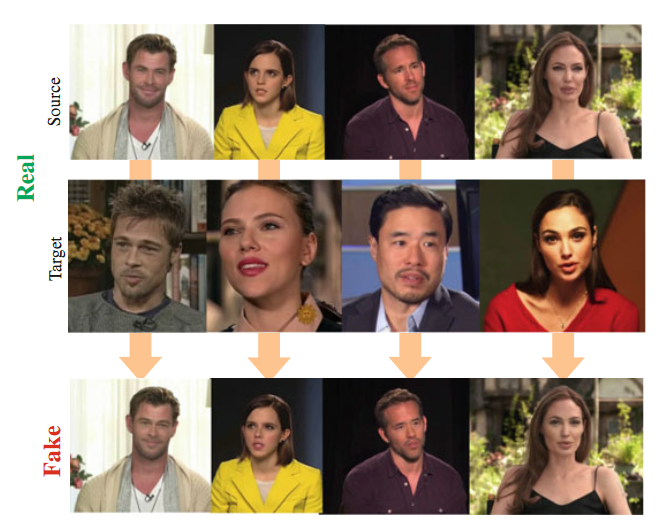
\includegraphics[width=.53\linewidth]{other-fig/idenity_swap.png}
    \caption{Examples of real and fake identity swap images. Retrieved from~\cite{IntroductionToDigitalFaceManipulation}.}
\label{fig:idenity_swap}
\end{figure}

\item Full puppet – Method related to identity swap allows creation of so-called puppet. One person (master) is source of facial expression and body movements that are mapped onto target person as shown in Fig.~\ref{fig:full_puppet}.~\cite{IncreasingThreatofDeepfakeIdentites}
\begin{figure}[H]
    \centering
    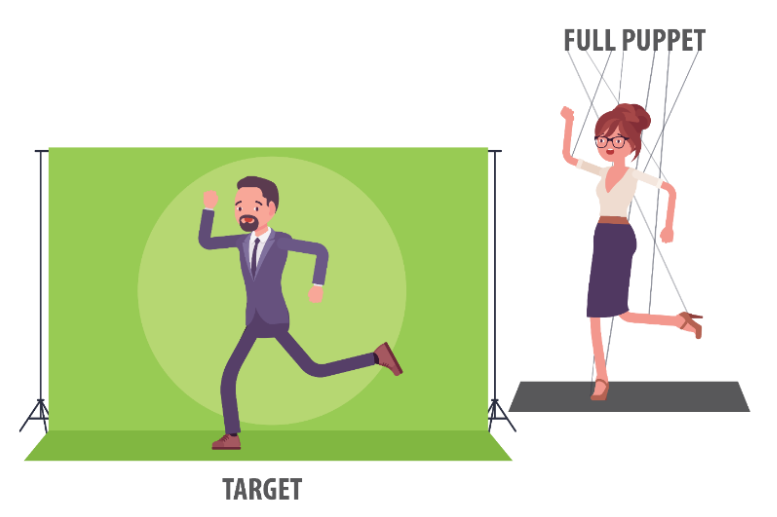
\includegraphics[width=.41\linewidth]{other-fig/full_puppet.png}
    \caption{Full puppet technique visualisation. Retrieved from~\cite{TheThreatOfDeepfakes}.}
\label{fig:full_puppet}
\end{figure}

\item Morphing – It is a type of manipulation that is used to create artificial biometric face samples. Final face contains resemble biometric information of two or more individuals. It should be possible to be successfully verified by biometrics systems for all individuals who were source for given deepfake. Fig.~\ref{fig:morphing} shows an example of a morphed image.
\begin{figure}[H]
    \centering
    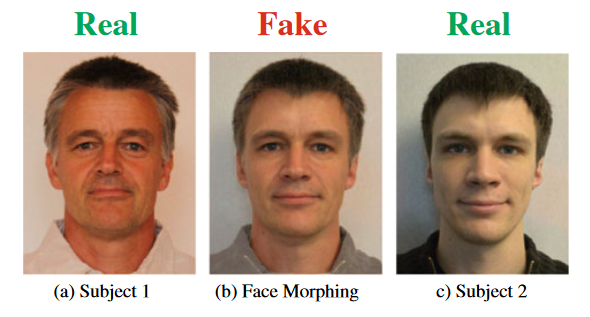
\includegraphics[width=.45\linewidth]{other-fig/morphing.png}
    \caption{Examples of fake morphed identity from Subject 1 and Subject 2. Retrieved from~\cite{IntroductionToDigitalFaceManipulation}.}
\label{fig:morphing}
\end{figure}

\item Attribute manipulation – Face editing or face retouching technique involves modifying some attributes such as length or color of hair, color of skin, sex, age, adding glasses or other artefacts, and more. Fig.~\ref{fig:attribute_manipulation} shows an example of this technique.
\begin{figure}[H]
    \centering
    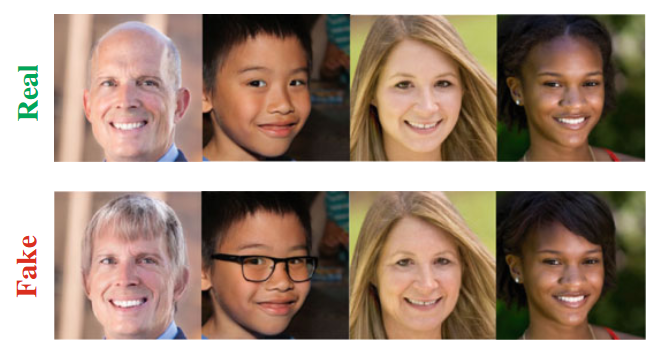
\includegraphics[width=.52\linewidth]{other-fig/attribute_manipulation.png}
    \caption{Examples of real and fake attribute manipulation category. Retrieved from~\cite{IntroductionToDigitalFaceManipulation}.}
\label{fig:attribute_manipulation}
\end{figure}

\item Expression swap – Modifying facial expression of the subject as shown in Fig.~\ref{fig:expression_swap}. This technique is used as one of part for full puppet.
\begin{figure}[H]
    \centering
    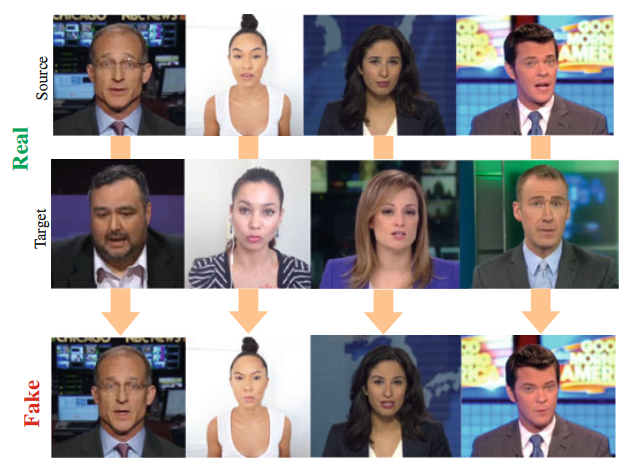
\includegraphics[width=.52\linewidth]{other-fig/expression_swap.png}
    \caption{Examples of real and fake expression swap category. Retrieved from~\cite{IntroductionToDigitalFaceManipulation}.}
\label{fig:expression_swap}
\end{figure}

\item Audio/text to video – This method related to expression swap synthesising facial expression from audio or text. It is also known as lip-sync deepfakes. Diagram in Fig.~\ref{fig:audio_to_video} shows how this method works.
\begin{figure}[H]
    \centering
    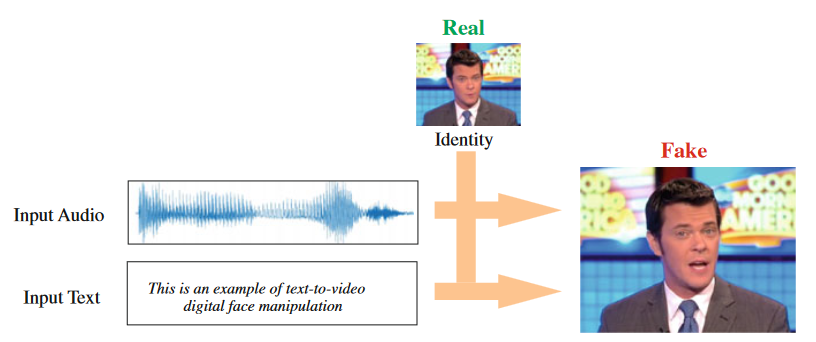
\includegraphics[width=.6\linewidth]{other-fig/audio_to_video.png}
    \caption{Examples of real and fake audio/text to video fake category. Retrieved from~\cite{IntroductionToDigitalFaceManipulation}.}
\label{fig:audio_to_video}
\end{figure}
\end{itemize}

Creating deepfakes nowadays is complex task and many deepfakes is using more techniques so that they could be included into more than one category. Attackers could create deepfake that will fall under identity swap category and after that use attribute manipulation to tune final results.

\chapter{Deepfake detection}
\label{chapter:deepfake_detectoin}

As we stated, humans are not good at recognizing deepfakes. Creating deepfakes could leave visible defects (e.g. blurring or misalignment on edges in the image). A. Firc~\cite{ApplicabilityOfDeepfakes} summarizes the list of features to focus on when spotting fakes for humans.

\begin{itemize}
\item Facial features – eyes and their movement, eyebrows, glasses, facial expression, hair and facial hair, skin, lips, teeth
\item Body features – body position and posture, body movements
\item Voice features – unusual tempo, end of words, fricatives, conversation
\item General indices – blurring or misalignment on edges, inconsistence noise or audio
\end{itemize}
	
This list points to critical parts where defects, which were created during the creation of deepfake, could be spotted. Generation of deepfakes is getting better, plus other masking techniques are being used. The big problem for detection is lossless compression, several chained resizes of an image, application of noise, etc. Basically, all methods that lead to some degree of data loss but without noticeable change for the naked eye or ear. When generation of deepfakes is not good enough manual post-processing could be used for polishing results (images – Photoshop, GIMP, etc.). 

Machine detection could be divided into two categories: standard algorithms looking for physical inconsistency and digital integrity, using the same features as Firc described. Other methods are based on machine learning. The same “masking” techniques listed before (compression, chained resizes, etc.) have the same effect on machine-based detection. Any data loss prevents the usage of reliable methods such as frequency analysis. Still, computers perform better than humans because they can also use different features (e.g., pixel-level features), especially neural networks trained for deepfake detection. ~\cite{MediaForensicsandDeepFakes}

The problem of neural networks is that we do not know what it is learnt to detect. It depends highly on training dataset. Probably the worst case scenario would be only recognizing suspicious images containing traces after “masking” techniques such as double compression, noise patterns, etc.

Another problem of detection algorithms is bad generalization. Most of methods are trained on single domain deepfake (e.g. identity swap), which means they are not able to recognize deepfake from different category. When methods are trained on multi-domain datasets, accuracy is going down.~\cite{FacialRetouchingAndAlterationDetection}

\section{Image/Video detection methods}

As stated, before most of methods for deepfake detection are targeting only single domain. This section will describe examples of proposed detection methods for image/video deepfakes. There are more conventional approaches and also more “exotic”.

P. Majumdar, et al. referring to multiple detection methods for image retouching (makeup, filters) and alternation (fully synthetize faces, morphing)~\cite{FacialRetouchingAndAlterationDetection}. Most of them use the same pattern which could be described as specific feature extraction followed by support vector machines (SVM) for classification. One of the methods proposed detection of images using face patches as input in the deep Boltzmann machine for feature extraction and SVM for binary classification. Another method uses softmax probabilities as features in the SVM. Other methods, for example, using convolutional neural networks.~\cite{FacialRetouchingAndAlterationDetection}

L. Spreeiwers, et al. made research on using local binary pattern with SVM for morphing detection~\cite{PracticalEvaluationOfFaceMorphingAttackDetectionMethods}. A single LBP histogram contains 59 feature values, which means that for a 3 × 3 layout, the feature space has 531 dimensions. The SVM classifiers are trained on between 650 and 1,000 samples. They also stated that EER increases to above 20 \% while adding Gaussian noise to the deepfakes images.

Non-conventional detection method is heart rate estimation (remote photoplethysmography) by J. Fierret~\cite{DetectionBasedOnHeartRateEstimation}. They are trying to estimate heart rate from video and evaluating frame-by-frame. There are other human physiological processes that could for be used instead heart rate such as blood oxygen or breath rate. The score oscillates during the video and final decision is based on the mean/median/QCD score.

There are many other methods, and each will have its pros and cons, but as we can observe, SVM classification with large range of different feature extractors. Another rising group of detectors is using CNN. There are not many researches using CNN as SVM but results seems to be promising as we can see in researches~\cite{3DCNNArchitecturesAndAttentionMechanismsForDeepfakeDetection}~\cite{CapsuleForensicsNetworksForDeepfakeDetection}.

\section{Voice detection methods}

Voice detection complicates different languages; it is similar story to image/video deepfakes. There are face swaps, morphing, etc., and for voice there are different languages and dialects. Voice detection methods also copying trend from image/video detection methods. Support vector machines (SVM) with different feature extractors or CNNs.

Z. Almutairi and H. Elgibreen refer to multiple methods~\cite{ReviewOfModernAudioDeepfakeDetectionMethods}. One of them uses the SVM model with Random Forest to predict synthetic voices based on a feature called Short-Term Long-Term. In this research, they compared SVM with many other classifiers such as Linear Discriminant, Quadratic Discriminant, Linear SVM, weighted K-Nearest Neighbors, and SVM outperforms all of them. Other referred work uses combination of two CNN, 1-D CNN and Siamese CNN. The Siamese CNN contained two identical CNNs that were the same as the 1-D CNN but concatenated them using a fully connected layer with a softmax output layer.~\cite{ReviewOfModernAudioDeepfakeDetectionMethods}

\section{Analysis of existing tools for detecting deepfakes}

Tools for deepfake detection are slowly getting from command line tools for experts to online tools with user-friendly interface. There are not many tools of this kind and some of them are not free to use. The following lines describe two available tools in a market.

\subsection{Deepware}

The Bosnia and Hercegovina recognize danger of deepfakes, while their parent company researched methods to develop an AI-based antivirus engine. Deepware company was founded to develop scanner for deepfake recognition.

Deepware provides REST API with web UI \footnote{\url{https://scanner.deepware.ai/}}, mobile android application. The backend of this project with pre-trained models is accessible on their GitHub as Python command line tool \footnote{\url{ https://github.com/deepware/deepfake-scanner}}.

\begin{figure}[H]
    \centering
    
\includegraphics[width=.65\linewidth]{other-fig/deepware_input.png}
    \caption{Deepware scanner input form}
    \label{fig:deepware_input}
\end{figure}

\begin{figure}[H]
    \centering
    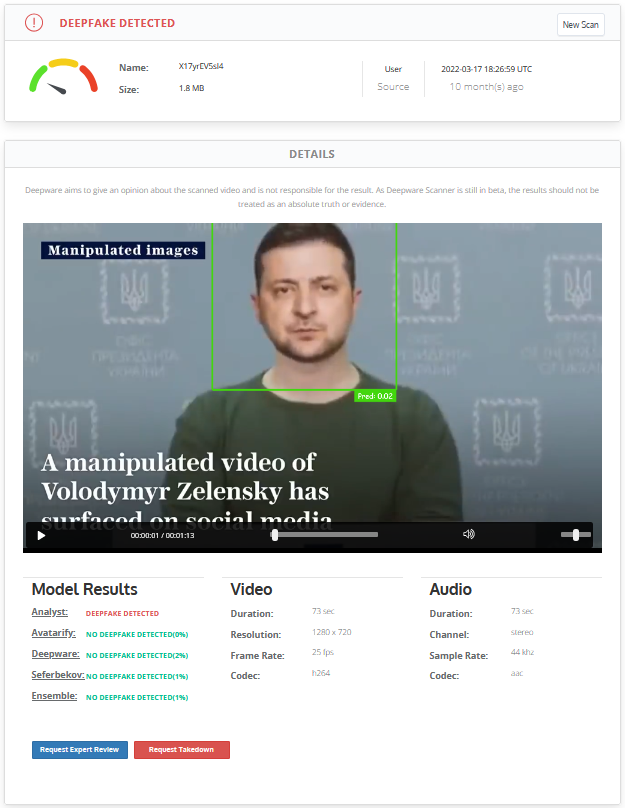
\includegraphics[width=.58\linewidth]{other-fig/deepware_results.png}
    \caption{Results of Deepware scanner containing probability of deepfakes from multiple detection methods}
    \label{fig:deepware_results}
\end{figure}

The Web application is stating that the project is in Beta, but unfortunately the last commit to the GitHub repository was made on 7th of June 2022 reported at the time of writing this thesis.

The tool provides a simple user interface to scan only videos. The user can input the link to the video (e.g. YouTube) or upload the video file directly as shown in Fig.~\ref{fig:deepware_input} . There are many supported video formats. The only limitation is the length of the video, which does not have to be longer than 10 minutes.

Processing of approximately 1 minute long video takes several seconds (3-10 seconds). Results contains video and audio metadata, results of multiple detection methods/models, and deciding whether it is a deepfake or not with gauge chart of confidence as we can observe in Fig~\ref{fig:deepware_results}. To use their Rest API, you need to request authentication token. API provides the same functionality as web UI via three methods.

\begin{itemize}
\item POST /video/scan
\item GET /url/scan
\item GET /video/report
\end{itemize}

The first two methods execute scan on a video file or link and return report ID. Results report could be retrieved by last method and results are returned as JSON. Documentation also code samples for multiple programming languages on how to use API properly. The provided API can be integrated to other processes like mail communication scans or file upload filters.

\begin{table}[H]
    \centering
    \begin{tabular}{|l|r|r|r|}
    \hline
     & \multicolumn{1}{l|}{\begin{tabular}[c]{@{}l@{}}Correct\\ (deepfake/original)\end{tabular}} & \multicolumn{1}{l|}{\begin{tabular}[c]{@{}l@{}}Incorrect\\ (deepfake/original)\end{tabular}} & \multicolumn{1}{l|}{Scan failed} \\ \hline
    Celeb DF & 10/7 & 0/0 & 3 \\ \hline
    FaceForensics++ & 4/5 & 1/0 & 10 \\ \hline
    \end{tabular}
    \caption{Deepware manual testing results}
    \label{table:deepware}
\end{table}

Deepware did not provide requested API key, so in table \ref{table:deepware} you can find results of manual testing. The test contains 40 videos from two different deepfakes datasets (20 from CelebDF and 20 from FaceForensics++). The distribution between original and deepfakes was 1:1. The accuracy of detection is decent, but from 40 tested files 13 files did not go through scan, even repeatedly. It is a very small sample, so we leave it to the reader to draw conclusions.

\subsection{Sensity}

Sensity is very similar from the user perspective to Deepware. Based on the post on Sensity blog~\cite{HowToDetectADeepfakeOnline} from 2021 we can explore web UI of their application. The application is not publicly accessible and to obtain access, you need to request it. Sensity provides more tools related to cybersecurity, person identification, and verification. 

Sensity allows for detection of images and videos by inserting files or referencing them via a URL link as shown in Fig.~\ref{fig:sensity_input}. Sensity allows processing of quite small group of file types (png, jpeg, jfif, tiff, mp4, mov). Another limitations are for videos regarding their size (up to 30MB), length (10 minutes), and quality of videos (1440p).~\cite{HowToDetectADeepfakeOnline}

\begin{figure}[H]
    \centering
    
\includegraphics[width=.95\linewidth]{other-fig/sensity_input.png}
    \caption{Sensity deepfake detection tool input form. Retrieved from~\cite{HowToDetectADeepfakeOnline}.}
    \label{fig:sensity_input}
\end{figure}

The tool is capable of recognize only face swap and fully synthesized faces by GAN. It is not able to recognize morphed images or other deepfakes. For GAN-genereated faces, it is sometimes able to classify model generator. If deepfake is recognized tool show how confident he is, all shwon in Fig.~\ref{fig:sensity_results}. Compared to Deepware, it provides image scans; on the other hand, it does not have mobile application.

\begin{figure}[H]
    \centering
    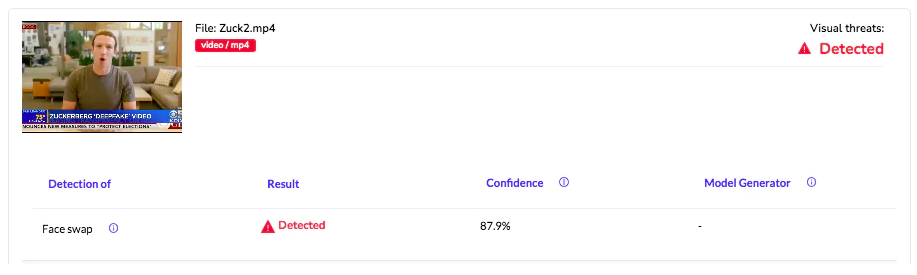
\includegraphics[width=.95\linewidth]{other-fig/sensity_results.png}
    \caption{Sensity deepfake detection tool results. Retrieved from~\cite{HowToDetectADeepfakeOnline}.}
    \label{fig:sensity_results}
\end{figure}

\subsection{Other}

Below you can find a list of other open source detection methods. These methods usually require a good knowledge of information technologies and programming to make them work on your computer. There is no guarantee that these methods really work, but two projects were selected for integration into the framework arising in this work.

\begin{itemize}
    \item Video
    \begin{itemize}
        \item dfdc\_deepfake\_challenge \\ (\url{https://github.com/selimsef/dfdc_deepfake_challenge})
        \item DeepFake Detection \\ (\url{https://github.com/dessa-oss/DeepFake-Detection})
        \item fakeVideoForensics \\ (\url{https://github.com/bbvanexttechnologies/fakeVideoForensics})
        \item Deepstar \\ (\url{https://www.zerofox.com/deepstar-open-source-toolkit/})
    \end{itemize}
\end{itemize}
\clearpage
\begin{itemize}
    \item Audio
    \begin{itemize}
        \item AudioDeepFakeDetection \\ (\url{https://github.com/MarkHershey/AudioDeepFakeDetection})
        \item specrnet \\ (\url{https://github.com/piotrkawa/specrnet})
    \end{itemize}
\end{itemize}

\chapter{Architecture and technologies analysis}

The goal of this work is to develop a deepfake detection framework capable of serving various client applications and an exemplary web plugin that communicates with framework and clearly displays the results to the user. We already analyze the market and test existing tools. Because there is no external contracting party defining their need, we will define requirements by ourselves. Requirements will be divided into two categories, functional and non-functional requirements. It is important to define not only functional logic, but also some limits on processing time, number of users, etc.

\section{Requirements}

As we already said, the framework has to support multiple clients, so there needs to be a properly defined communication interface between the client applications and the framework itself, which will act as server in this case. Framework allows dynamic changing detection methods, which means it is able to add, remove, or edit detection method. This implicates multiple detection methods at one time for image, video, and even voice deepfake detection. Editing detection method means updating the model or constant parameters. 

The platform should support as many file types as possible and adding a new method should not affect methods already presented in the framework, within supported file types. Different detection methods have different models depending on their design, so model management will be wrapped completely into the detection method.

The framework should collect statistics and hardware metrics, but the collection of personal information should be omitted. All collected metrics will be used for future improvements of detection methods and optimizing operating costs and performance. We would like to have a short response time with as low operating costs as possible. Those two parameters are in contradiction, so there has to be some balance between them. Scalability of the framework or some computationally intensive parts of the framework will help with these requirements. From a perspective number of users, the platform will handle up to hundreds of users at one time, and with enough resources the framework should handle even more.

The client application has to be simple so that anyone can use it. Users should be able to upload files or put a link to a file. The Web plugin allows access to DOM of the webpage so an optional extension will be selection of web elements and retrieval from metadata of it automatically. Because it should cover a large group of possible users, results have to be easy to understand and also provides information for experienced users. Last but not least, the client application should enable users to send feedback. There are several web browsers in market that cover almost all audience, it will be nice that the developed web plugin will be portable among multiple web browsers.

Today it is standard, but it is necessary to mention that the application should be secured. It will affect code of framework, client application, and environment itself (hardware, operating systems, …). All work is open-source and accessible on the public GitHub repository.
\\\\
\noindent Summary of functional requirements:
\begin{itemize}
\item Adding, removing, and editing (changing parameters and models) detection methods
\item Multiple detection methods at once
\item Collecting statistics and feedback
\item Detection of image, video, and voice
\item Detection of file, URL link, or selected HTML element (optional)
\item Understandable presentation of results
\item Security
\end{itemize}

\noindent Summary of non-functional requirements:
\begin{itemize}
\item Scalability
\item Small response time
\item Low operating costs
\item Portability of the web plugin among multiple web browsers (optional)
\item Open source
\end{itemize}

\section{Containerazation}

The framework requires dynamic management of the detection methods. It means that the framework can contain one or twenty different detection methods. Each method could be developed using different programming languages or technologies. Also, model management will be integrated into the detection method. This leads to some isolation of each detection method with a defined communication protocol. Another requirement requires scalability of framework, and all this together will be reached via containerization.

There are many technologies dealing with containers, such as Docker, Podman, LXC. When we start counting orchestration with automatic scalability, the number of technologies drops down. Cloud solutions such as AWS, Azure offer Kubernetes for orchestration of Docker containers. In addition, Docker is probably the most widely used technology for containerization. Because of the huge community and good support of different cloud platforms, we can possibly run framework, we will stick with duo Kubernetes and Docker.

\section{Framework}

The framework is a collection of detection methods, an interface for the client application (receiving requests, sending report response), and orchestrates/arranges all communication. It will be built into several containers and one of the containers will be providing client application interface. It could be Rest API, GraphQL or custom protocol. It is not a good idea to develop a custom communication protocol, so we will stick to the most used Rest API. For this purpose, we can use a huge number of different technologies such as ASP.NET Core, Flusk, Django, Ruby on Rails, etc.

Basically all named technologies meet defined requirements (response time, number of users, ect.) because most of them are covered by microservice design and containerization described in chapter X. Our choice is ASP.NET Core because it has a huge community, Linux support, many external libraries, it is suitable for bigger projects, and it has good speed of program development.

\section{Web browser plugin}

Web plugins are based on web technologies such as HTML, CSS, JavaScript, TypeScript, etc. There are also technologies like WebAssembly which allow development of web applications in languages like C++ without usage of web framework. Because of portability and good integration we will choose HTML, CSS, and Typescript. Typescript is a strict syntactical superset of JavaScript and adds optional static typing to the language. It is also compiled into JavaScript. With those technologies we could be able to create portable web plugin for Chromium base browsers and Firefox.

\chapter{Framework architecture}

The architecture must reflect that each detection method could be developed in different architectures. We can isolate the detection methods from each other and wrap them into independent services. We do not need communication among all detection methods because they do not cooperate or share any data. In this case, the microservice architecture meets all defined requirements.

\section{Microservice architecture}

Microservice architecture is the style of developing applications. Example of design can be observe in Fig.~\ref{fig:microservice_architecture}. The microservice allows the application to be separated into smaller logical independent parts. The service then has its own realm of responsibility and they can communicate with each other. Containers are a well-suited microservice architecture example.~\cite{WhatIsMicroservicesArchitecture}

\begin{figure}[H]
    \centering
    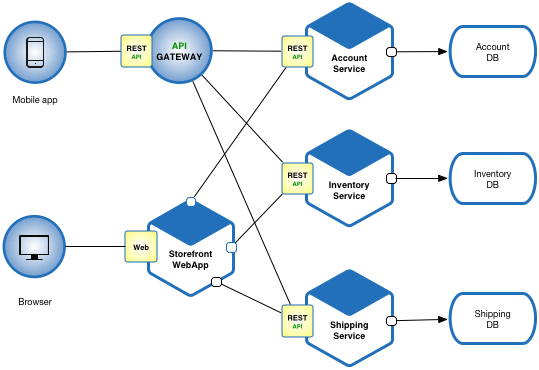
\includegraphics[width=.5\linewidth]{other-fig/microservice_architecture.png}
    \caption{Microservice architecture of fictitious e-commerce application}
    \label{fig:microservice_architecture}
\end{figure}

Microservices improve fault isolation that non-functional service should not affect others, in best case scenario. In real cases microservices depend on each other and this might lead to a problem. For example, if one service contains a memory leak, it is not propagated into other ones. Another benefit was already mentioned, and it eliminates commitment to one technology stack. One service has better maintainability because it should be small (better understandability, faster tools), which leads to more productive developers.~\cite{ MicroserviceArchitecture}

This architecture also has several drawbacks. It increases the complexity of architectural design and additional implementation of cross-service communication. When saving data to database, developers have to deal with distributed system because each service has its own independent database.~\cite{ MicroserviceArchitecture}

\section{High-level architecture}

The user communicates directly with the Rest API endpoint. This part of the design may be labelled as master process because it is handling request, preparing and validating data, selecting which type of processing should be used. After processing is done, it collects all results and distributes them back to the user. Fig.~\ref{fig:framework_architecture} contains high-level design of framework with data flow.

\begin{figure}[H]
    \centering
    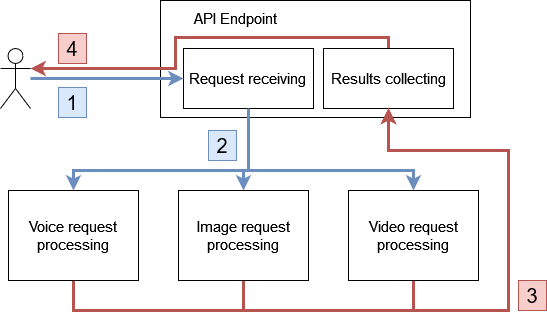
\includegraphics[width=.7\linewidth]{other-fig/framework_architecture.png}
    \caption{High-level design of whole framework}
    \label{fig:framework_architecture}
\end{figure}

The architecture separates voice, image, and video detection into an independent unit. Each unit contains a processing queue where the request will be assigned by the master process/Rest API. The queue is serviced by one or multiple processing units that contain all related detection methods as shown in Fig.~\ref{fig:framework_architecture_request_processing}.

\begin{figure}[H]
    \centering
    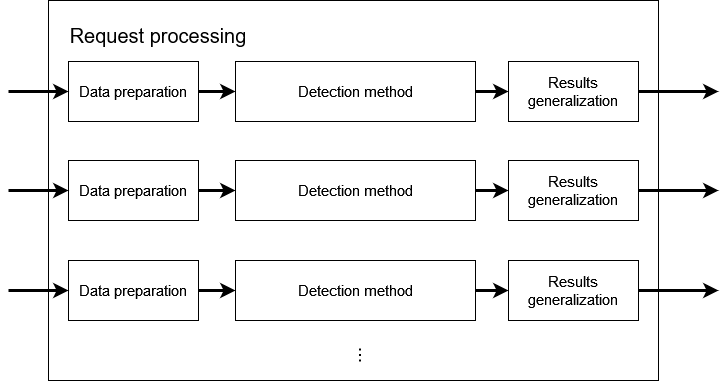
\includegraphics[width=.65\linewidth]{other-fig/framework_architecture_request_processing.png}
    \caption{Request processing detail}
\label{fig:framework_architecture_request_processing}
\end{figure}

The processing unit works as a parallel pipeline. Closer look at design is in Fig.~\ref{fig:framework_architecture_processing_unit}. Some detection methods require input data in specific format, so the first step is optional data preparation. Some methods are wrapping data preparation by themselves. The next step is the detection method that decides whether the input data contains deepfake or not. Detection methods are different, so are their results, so we need to properly generalize and also normalize them.

\begin{figure}[H]
    \centering
    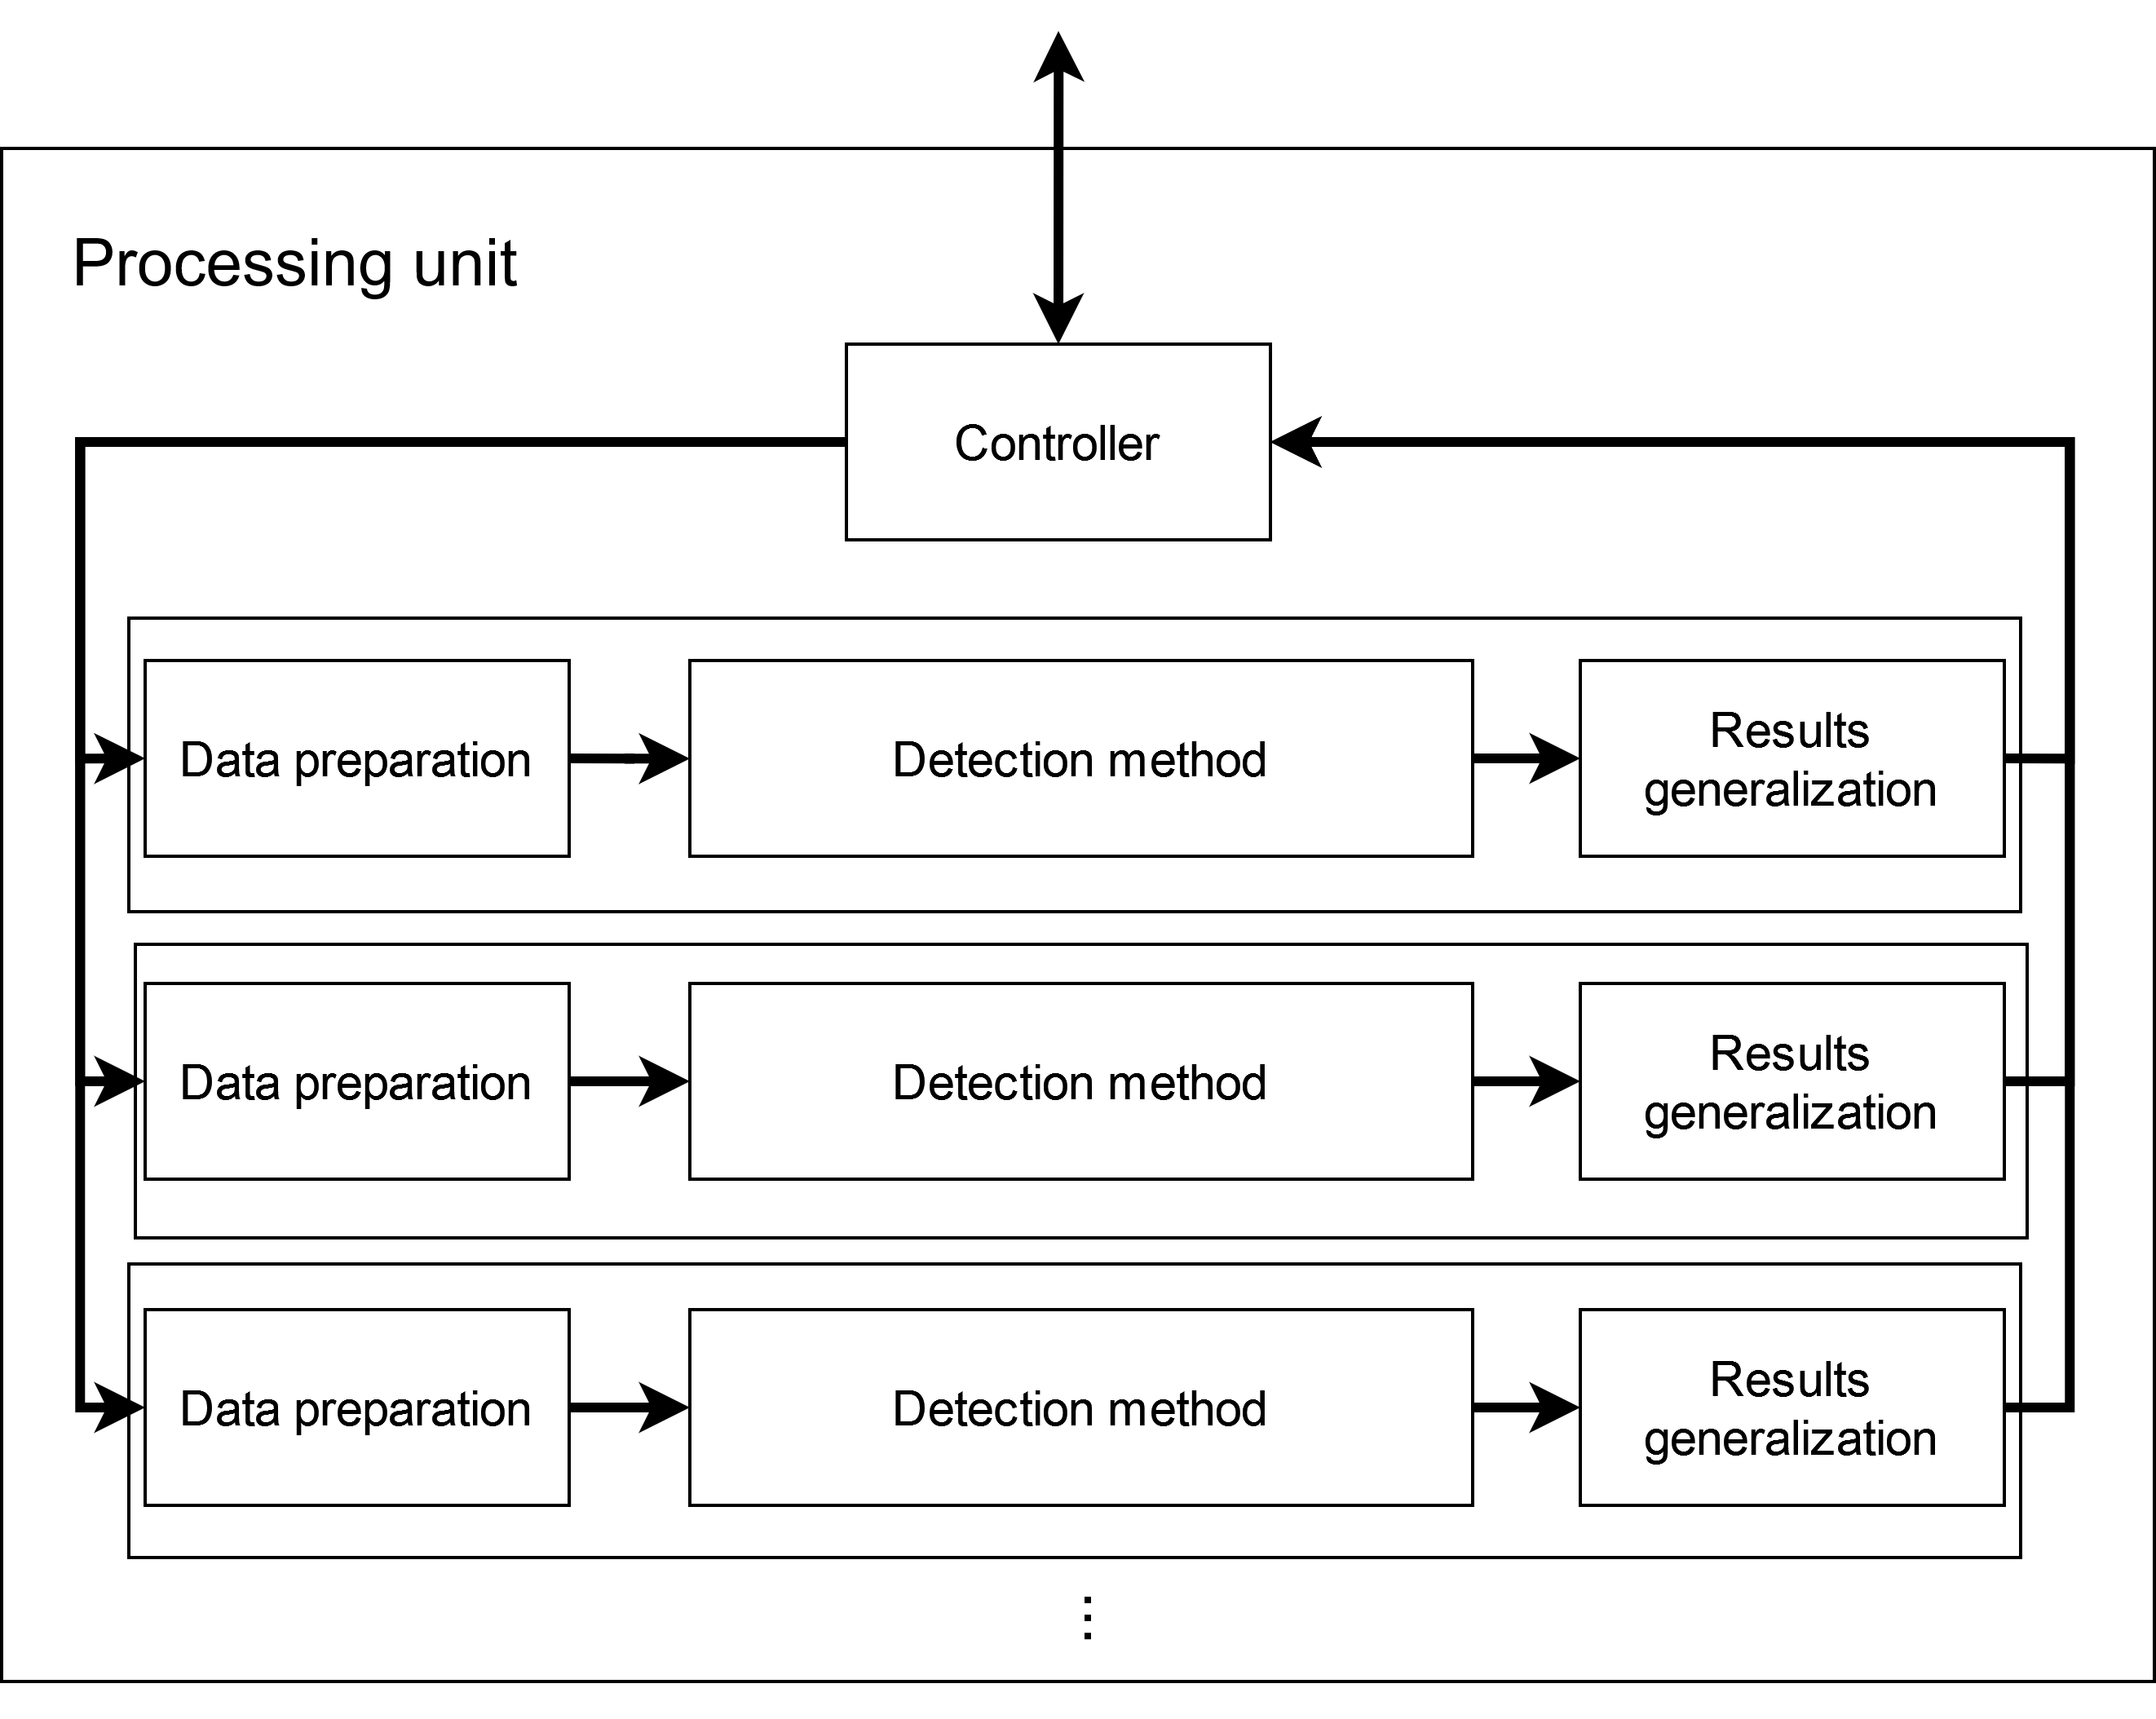
\includegraphics[width=.65\linewidth]{other-fig/framework_architecture_processing_unit.png}
    \caption{Processing unit pipeline}
\label{fig:framework_architecture_processing_unit}
\end{figure}

\section{Containerization and scaling}

Detection methods have to be containerized, and to decrease complexity data preparation and results generalization will be encapsulated together with detection method. The processing unit then will be the collection of containers/pods.

The processing unit then can be clone/scale up when needed to process more requests. Scaling up can be done automatically by setting specific rule in container orchestrator. To save costs we can scale down when a peek of request disappeared.

\section{API Endpoint}

As mentioned before, API endpoints communicate directly with user application and with backend processing mechanism. Processing takes same time, so user application creates request and wait asynchronously to be processed by the framework. The API for this purpose contains “detect” and “request” methods. “Detect” methods start processing and“requests” methods manage already running process. There are other support methods for possible health check or providing feedback. All methods are described in following list:

\begin{itemize}
\item /ping
    \begin{itemize}
    \item GET /ping – healtcheck endpoint
    \end{itemize}
\item /detect
    \begin{itemize}
    \item POST /detect/file – creates request with file in HTTP request body
    \item POST /detect/link – creates request with link to a file in HTTP request body
    \end{itemize}
\newpage
\item /request
    \begin{itemize}
    \item GET /request/stop/<request\_id> - stops running request
    \item GET /request/results/ – returns results of processed request or empty results if request is in process
    \end{itemize}
\item /feedback
    \begin{itemize}
    \item POST /feedback/<request\_id> - collects user feedback with optional parameter request\_id
    \end{itemize}
\end{itemize}

Each detection method has different processing times. There are two options to return results to user: partial results from the detection methods already completed or returns only when everything is completed. Because there is no need to show partial results, the second option will be used. This requires the use of another queue for respons or some sort of database. The framework needs to calculate the overall score and this requires all results from all methods. Calculating the total score requires considering the univariate methods as well as their domain differences. A single method will usually focus on a single domain (e.g. face swap). We leave the exact definition to the implementation section.

The method \texttt{/request/results} could be possibly replaced by websockets which will increase complexity, but on the other hand a user application could better report status of the running process. It is one of the possible extensions to the framework.

\section{Request processing and processing unit}

API endpoint placing all new requests in the request queue. One of the available processing units takes the first request form queue. This request contains all the information such request ID, data for detection, and metadata for this data.

The first step in the processing pipeline is optional data preparation. The detection method could be trained only on a specific resolution of the video/image or on a specific length of the voice sample. This means data processing unit has to be designed for a given detection method. When data are prepared for detection, they continue to the detection unit.

After detection, the same case as optional data preparation is optional data generalization/normalization. Because results need to the be correctly presented to user and the framework needs to calculate over all scores, all results need to the be normalized to same scale and “units”. When results contain more specific information, in this case it needs to be generalized. Results could contain field with additional/extra information about results which could also be presented to the user. Results are then pushed to the results queue or database, depending on implementation.

\chapter{Client architecture}

The use case of the client application is straightforward, so there does not need to be use case or data flow diagrams. The application will try to prepare the file for inspection and send it to the server framework. The next section contains several wireframes of how the client application should look like with description.

\section{Web browser plugin}

It should allow the user to insert a file via file upload, link, or HTML element containing a targeted file. In Fig.\ref{fig:client_wireframe_input_selection} we can see type insertion selection, for file upload the user will be prompted by system file upload picker. When user pick link as input, floating windows will pop up, and user then can insert URL to file. Those two selections are the same as other tools in market also provide. Optional improvement will be element selection which switches the application to interactive mode where user can point to HTML element and application will try to retrieve metadata of image or video directly from HTML. 

\begin{figure}[H]
    \begin{subfigure}[h]{.5\linewidth}
        \centering
        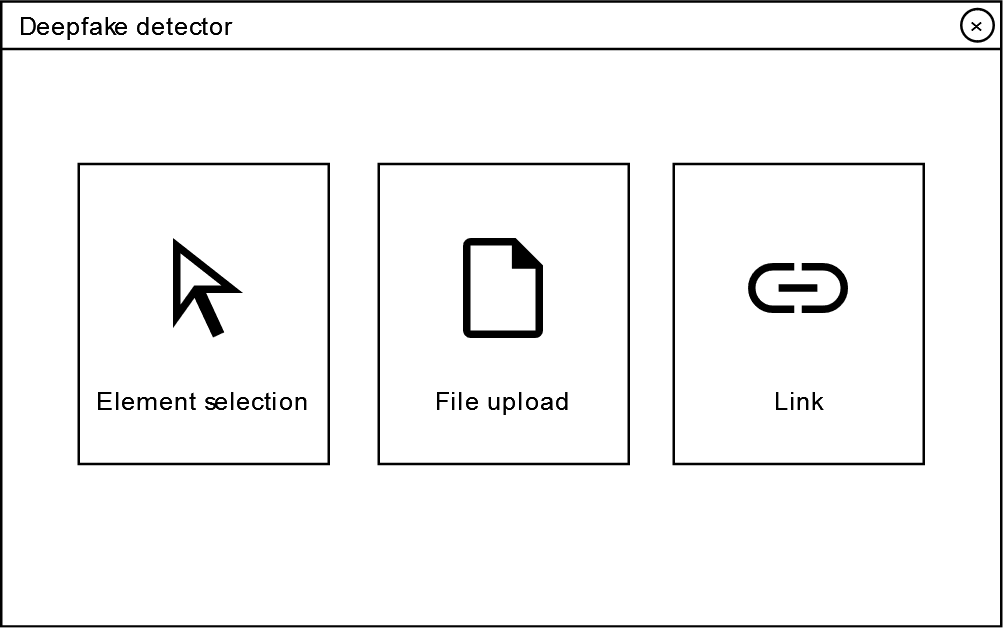
\includegraphics[width=1\linewidth]{other-fig/client_wireframe_input_selection.png}
        \caption{Input type selection}
    \end{subfigure}
    \hfill
    \begin{subfigure}[h]{.475\linewidth}
        \centering
        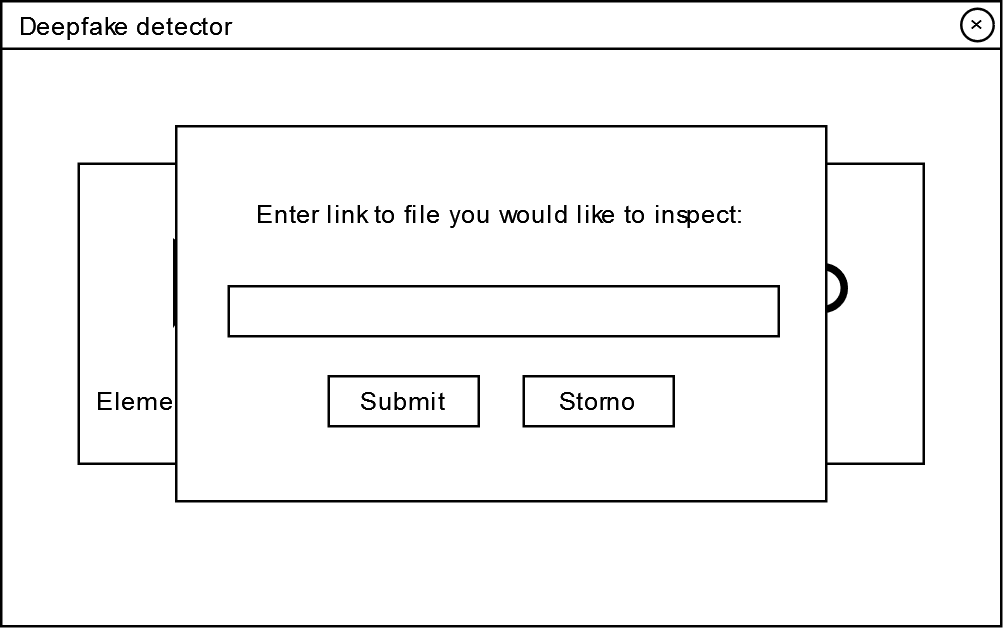
\includegraphics[width=1\linewidth]{other-fig/client_wireframe_input_selection2.png}
        \caption{Link input in floating window}
    \end{subfigure}
    \caption{Input type selection screens}
    \label{fig:client_wireframe_input_selection}
\end{figure}

Because detection framework will contain several detections method we need to show the result of each method independently. It could be a little confusing for user so there will also be overall score which interprets/generalizes all the results of each method. The overall score will indicate the results as a percentage and as emoticon. The palette will contain four emoticons shown in Fig~\ref{fig:client_wireframe_results3}. For better understanding there are question marks in the UI that after mouse hover shows tooltip with description. Whole results screen can be view in Fig.~\ref{fig:client_wireframe_results}.

\begin{figure}[H]
    \begin{subfigure}[h]{.475\linewidth}
        \centering
        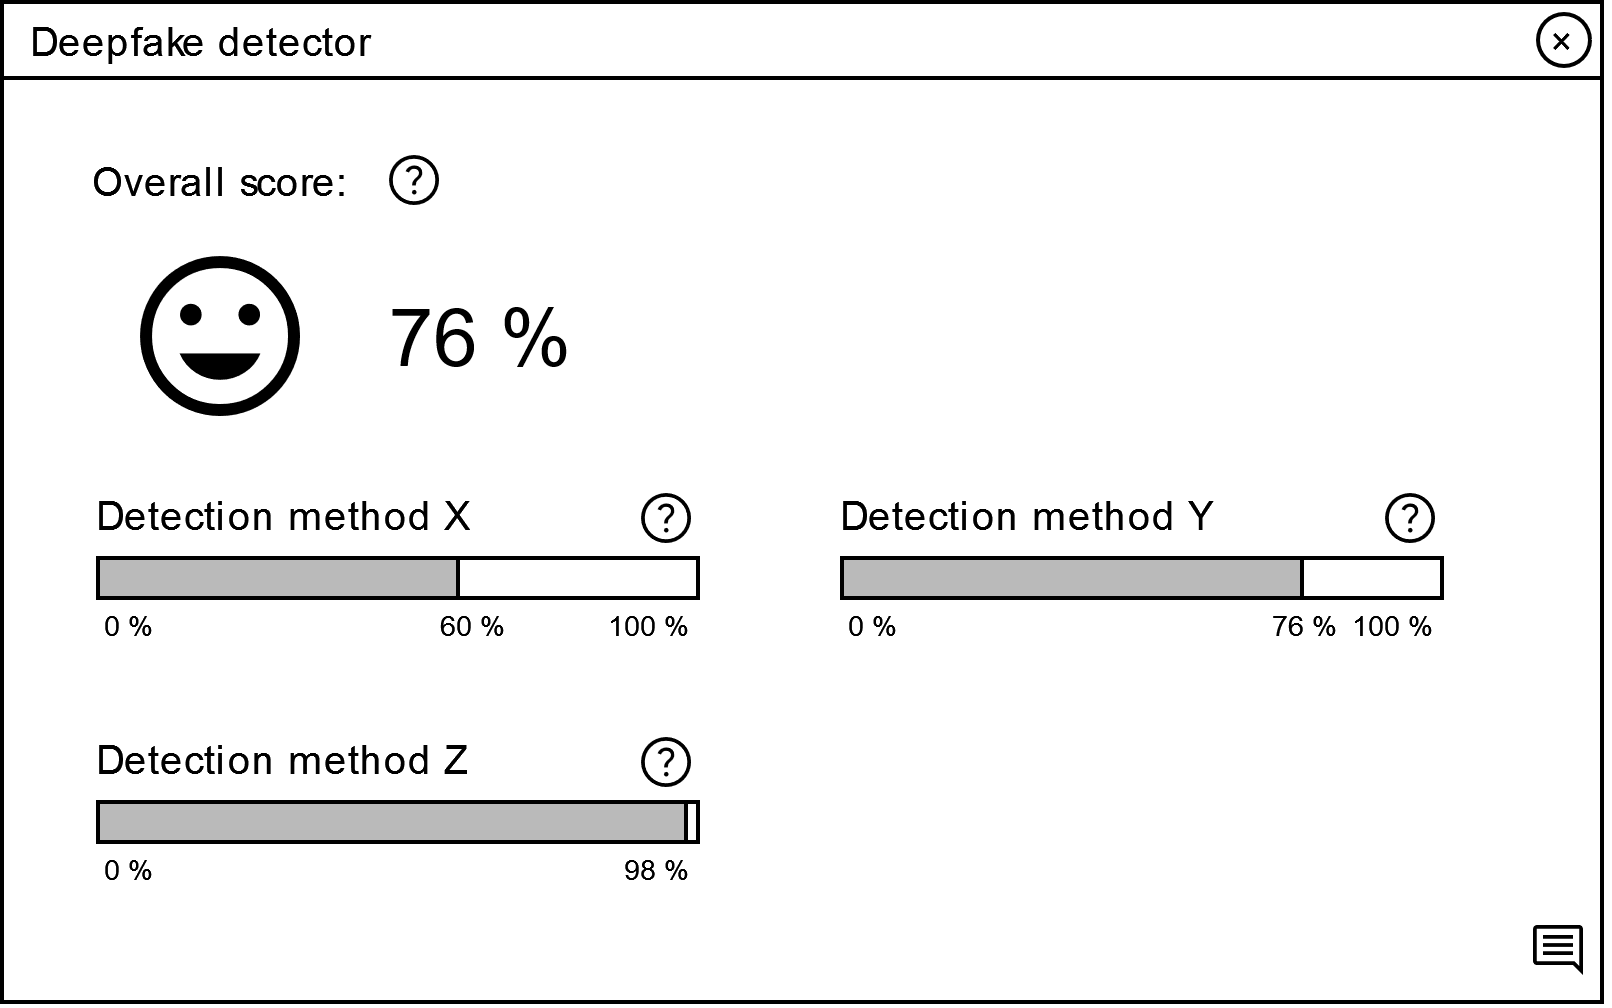
\includegraphics[width=1\linewidth]{other-fig/client_wireframe_results.png}
        \caption{Results view}
    \end{subfigure}
    \hfill
    \begin{subfigure}[h]{.475\linewidth}
        \centering
        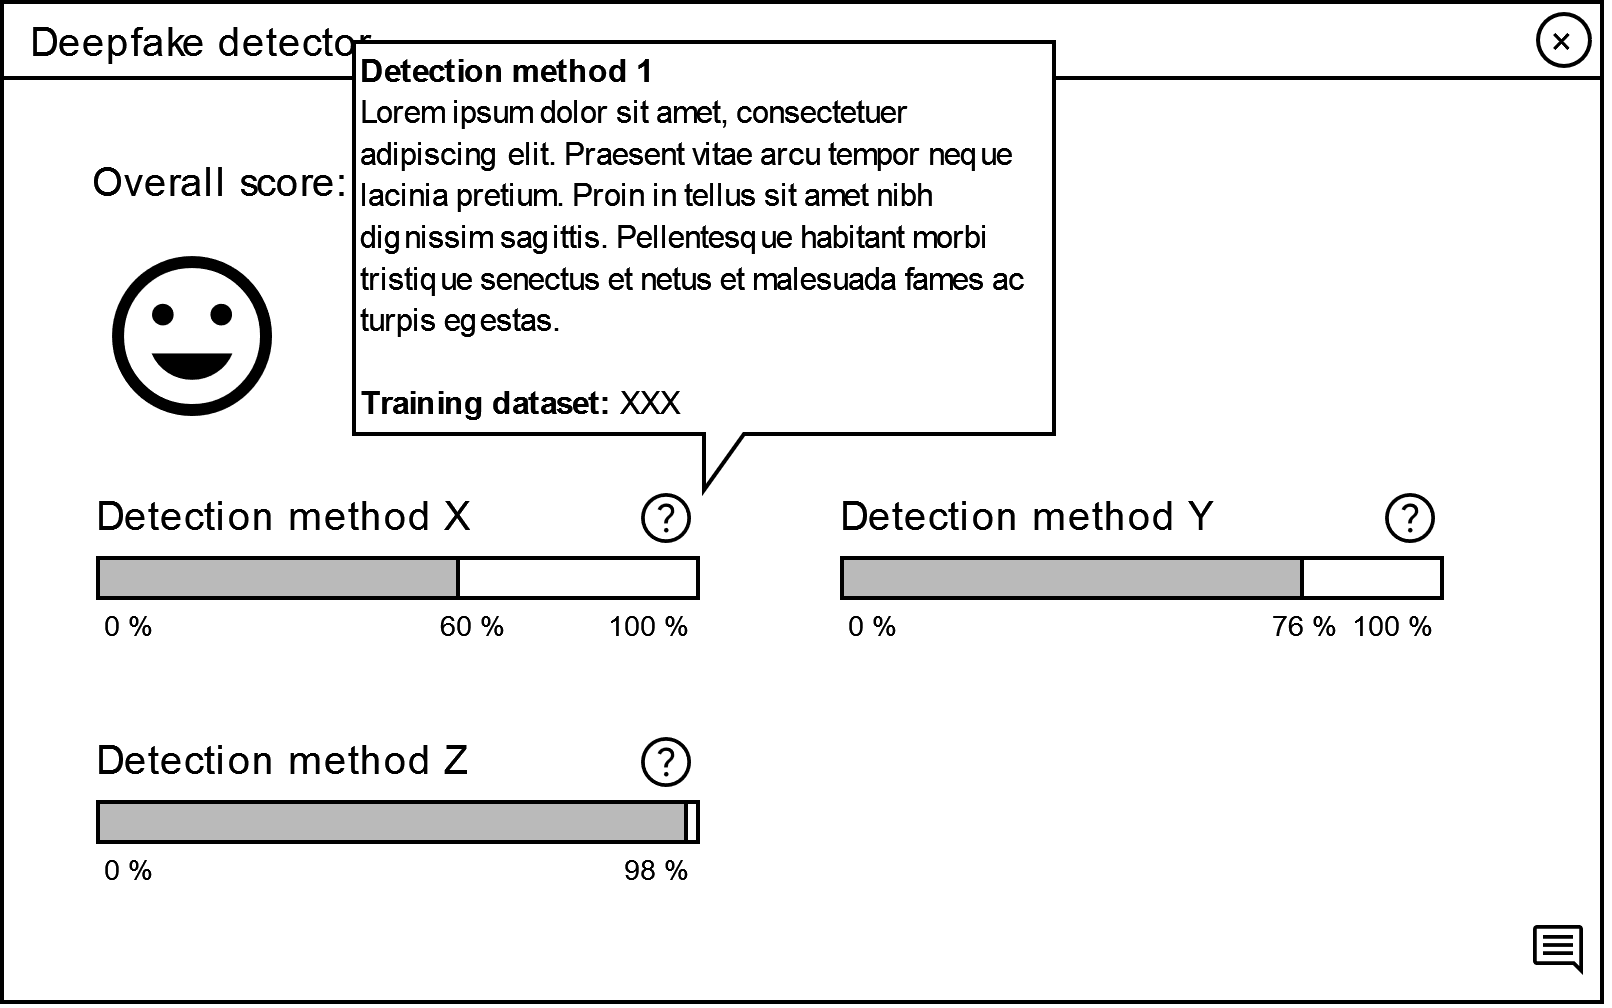
\includegraphics[width=1\linewidth]{other-fig/client_wireframe_results2.png}
        \caption{Tooltip showing description one of detection method}
    \end{subfigure} 
    \caption{Results view screens}
    \label{fig:client_wireframe_results}
\end{figure}

\begin{figure}[H]
    \centering
    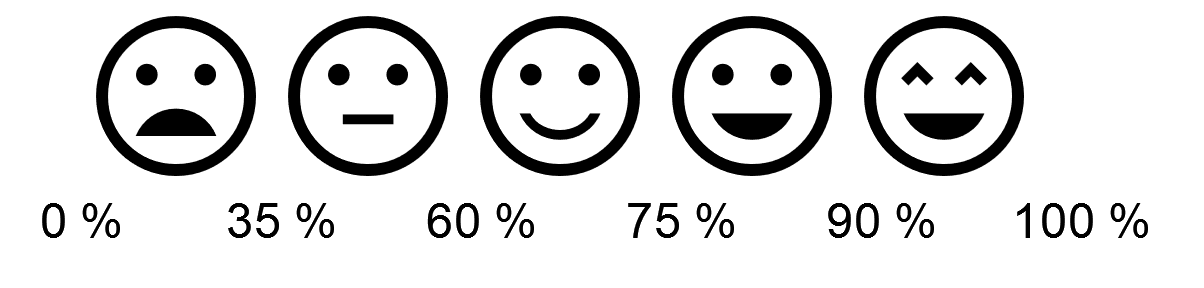
\includegraphics[width=.4\linewidth]{other-fig/client_wireframe_results3.png}
    \caption{Palette of emoticons indicating if inspected file contains deepfake or not}
\label{fig:client_wireframe_results3}
\end{figure}

At the bottom of each screen there is an icon that enables the user to the send feedback to application. After clicking on this icon floating window will appear, shown in Fig~\ref{fig:client_wireframe_feedback}. When user will be sending feedback on the result page, the internal result ID will be added as an additional parameter to the feedback message. 

\begin{figure}[H]
    \centering
    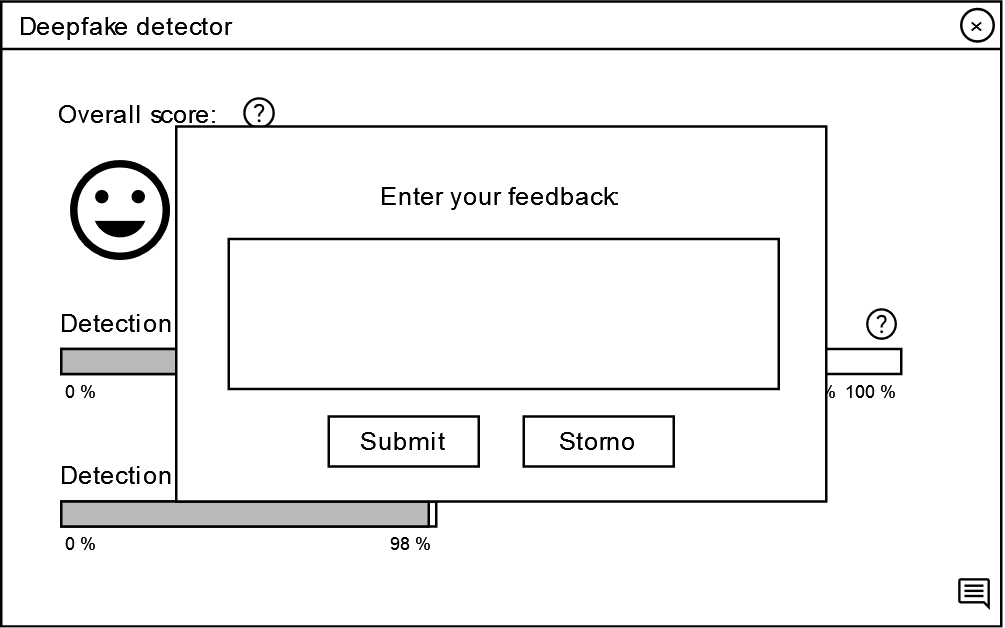
\includegraphics[width=.475\linewidth]{other-fig/client_wireframe_feedback.png}
    \caption{Feedback form in floating window}
\label{fig:client_wireframe_feedback}
\end{figure}

\chapter{Framework implementation}
...
\section{API endpoint}
ASP.NET Core + EF Core; file checksums, communication, deployment ...
\section{Message broker}
RabbitMQ, how it works, deployment
\section{Processing unit}
Controller + detection method communincation, deployment
\section{Monitoring}
Prometheus, Grafana - metrics scraping, what is collected and why
\section{Scalability}
Prometheus adapter, horizontal pod autoscaler based on metrics
\section{Detection method integration}
how to integrarte new method; what is required from container with detection methode; what manifests needs to be change + caution about detection method resources

\chapter{Selected detection methods}
...
\section{AudioDeepFakeDetection}
train 6 differnet methods (LJ + WaveFake dataset); results of training; automaticlly spliting dataset; own implementation of evaluation of one file; dockerfile optimalization
\section{fakeVideoForensics}
used pretrained model (no description how to train); dockerfile optimalization

\chapter{Client application implementation}
angular + angular materials
\section{Functionalities}
element selection not implemented, file upload + link is working 
\section{Communication with framework}
pooling messages with timeout
\section{Supported browsers}
tested in chrome, firefox (working but not able to upload file because of bug in browser) and edge

\chapter{Test experiment and results}
...
\section{Datasets}
which datasets were used for testing (CelebDF, FaceForensics++, LJ + WaveFake, ASV2021) - how was subset created; stats - size, count
\section{Test case 1 - accuracy}
accuracy of detection methods - 4x (250 originals + 250 fakes) - results no so good...
\section{Test case 2 - small bursts}
small burtst (100 files - batches of 5) - resources (cpu, ram), number of replicas, time
\section{Test case 3 - congestion}
small burtst (100 files - all in) - resources (cpu, ram), number of replicas, time
\section{Tests evaluation}
discussion about testing - detection methods not so good but it is replication on their experiment
\section{Cost analysis}
testing system - cpu, ram - average daily cost 

\chapter{Conclusion}
everythings implemented and it is working, :)